\documentclass[
  a4paper,
  twoside,
% oneside,
% openany,
  notitlepage,      %% Separate Titelseite (alternativ: titlepage)
  ngerman,          %% Das Dokument ist in neuen deutschen Rechtschreibung gehalten
  11pt,
% draft,            %% Finden von �berlangen Zeilen (dargestellt durch schwarze Bl�cke)
]{book}             %% Dokumentklasse (alternativ: article, report, etc.)
       
%% \linebreak f�r Zeilenumbruch
\usepackage[latin9]{inputenc}               %% Eingabezeichensatz zur Darstellung von Umlauten (latin1) erweitert um Sonderzeichen wie EURO (latin9)
\usepackage{csquotes}                       %%
\usepackage{times}                          %% Schrift Times
%\usepackage{mathpazo}                      %% Schrift Palatino
%\usepackage{luximono}                      %% Fette Schreibmaschinenschrift
\usepackage[a4paper]{geometry}              %%
\usepackage[hyphens]{url}                   %%
\usepackage{caption}
\usepackage{subcaption}                     %% Besser als subfigure und subfig
\usepackage{picins}                         %%
\usepackage{longtable}                      %%
\usepackage{shadethm}                       %%
\usepackage{amsmath}                        %%
\usepackage{framed, color}                  %%
\usepackage{fancyhdr}                       %%
\usepackage{lscape}                         %% stellenweises Querformat
\usepackage[T1]{fontenc}                    %% Europaeische Schriftcodierung (T1) und 
\usepackage{here}                           %% Grafik dort positionieren wo man es will ([H])Kopfzeile und Seitenzahlen
\usepackage[ngerman]{babel}                 %% => ngerman = neue deutsche Rechtschreibung
\usepackage{graphicx}                       %% Zur Einbindung von Grafiken. Z.B. ueber \includegraphics
\usepackage{listings}                       %% Codelistungs formatieren
\usepackage{chngpage}                       %% Seiteneinstellungen anpassen (adjustwidth)
\usepackage{paralist}                       %% flexible Listen
\usepackage{url}                            %% Darstellung von Internetadressen und Pfaden
\usepackage{setspace}                       %% zum Erzeugen von groesseren Zeilenabstaenden
\usepackage{nomencl}                        %% Abkuerzungsverzeichnis erstellen
\usepackage{tabularx}                       %% Tabellen mit fester breite nutzen
\usepackage{multirow}                       %% Zellen in Tabellen zusammenfassen
\usepackage[clearempty]{titlesec}           %% Keine Seitenzahlen, Kopf- und Fusszeilen auf leeren Seiten
\usepackage{savefnmark}                     %% Fussnoten mehrfach verwenden
\usepackage{colortbl}                       %% Farben in Tabellen
\usepackage{booktabs}                       %%
%\usepackage{hyperref}                       %% Phantomsection
\usepackage[backend=bibtex8]{biblatex}      %% "`Abgerufen am"' bei online quellen
\usepackage{eurosym}
\usepackage{placeins}                       %% floatbarrier
\usepackage{blindtext}                      %% lorem ipsumtext
\usepackage{nomencl}                        %% Abk�rzungsverzeichnis
%\usepackage[intoc]{nomencl}                 %% Abk�rzungsverzeichnis
\usepackage{xspace}                         %% nicht erzwungene Leerzeichen (f�r \newcommand n�tzlich}
\usepackage{todo}

%\onehalfspacing                             %% 1.5 Zeilenabstand
%\doublespacing                              %% Doppelter Zeilenabstand
%%%%%%%%%%%%%%%%% links %%%%%%%%%%%%%%%%%%%%%%%%%%%%%%%%%%%%%%%%%%
\usepackage[pdftex, pdfborder={0 0 0},colorlinks, linkcolor=black, citecolor=black, filecolor=black, urlcolor=blue, bookmarks=true, bookmarksnumbered=true]{hyperref}
%%%%%%%%%%%%%%%%%%%%%%%%%%%%%%%%%%%%%%%%%%%%%%%%%%%%%%%%%%%%%%%%%%

%-------------------------------------------------------------------------
%���Listings
%-------------------------------------------------------------------------

% Einstellungen f�r Listings mit Eclipse Code Style.
\usepackage{color}
\usepackage{courier}
\lstset{language=java}
\definecolor{sh_comment}{rgb}{0.12, 0.38, 0.18 }     % adjusted, in Eclipse: {0.25, 0.42, 0.30 } = #3F6A4D
\definecolor{sh_keyword}{rgb}{0.37, 0.08, 0.25}      % #5F1441
\definecolor{sh_string}{rgb}{0.06, 0.10, 0.98}       % #101AF9% Farbe f�r Kommentare
\def\lstsmallmath{\leavevmode\ifmmode \scriptstyle \else� \fi}
\def\lstsmallmathend{\leavevmode\ifmmode� \else� \fi}
\lstset {
  frame=shadowbox,
  rulesepcolor=\color{black},
  showspaces=false,showtabs=false,tabsize=2,
  numberstyle=\tiny,numbers=left,
  basicstyle= \scriptsize\ttfamily,
  stringstyle=\color{sh_string},
  keywordstyle = \color{sh_keyword}\bfseries,
  commentstyle=\color{sh_comment}\itshape,
  captionpos=b,
  xleftmargin=0.7cm, xrightmargin=0.5cm,
  lineskip=-0.3em, breaklines=true,
  escapebegin={\lstsmallmath}, escapeend={\lstsmallmathend}
}
\newcommand{\lstJava}[1]{\lstinline[language=Java,breaklines=true,basicstyle= \listingsfontinline]$#1$}
\newcommand{\lstXML}[1]{\lstinline[language=XML,breaklines=true,basicstyle= \listingsfontinline]$#1$}

\newcommand{\lstSetTiny}{\lstset{basicstyle= \scriptsize\tiny}}
\newcommand{\lstSetNotmal}{\lstset{basicstyle= \scriptsize\ttfamily}}
\newcommand{\lstSetBig}{\lstset{basicstyle= \ttfamily\mdseries}}

\newcommand{\lstSetJava}{\lstset{language=java}}

\newcommand{\lstSetXML}{\lstset{
  language=XML,
  morekeywords={encoding,
    xs:schema,xs:element,xs:complexType,xs:sequence,xs:attribute}
}}

%\usepackage{fontspec}                        %% Codelistungs formatieren
%\newfontfamily\listingsfontinline[Scale=0.8]{Courier New} 
%\newfontfamily\listingsfont[Scale=0.7]{Courier}


\bibliography{bibliography/bibliography}
\definecolor{shadecolor}{gray}{.65}
\definecolor{lightgrey}{gray}{.90}
\geometry{top=3cm, bottom=3cm, inner=4cm, outer=3cm}  %% Seitengroesse festlegen 

%%Einr�ckung bei neuem Absatz entfernen
\setlength{\parindent}{0pt}
\setlength{\parskip}\medskipamount % besser als explizite Angabe in pt

%%%%%%%%%%%%%%%%  Kopfzeile und Seitenzahlen %%%%%%%%%%%%%%%%%%%%%
\setlength{\headheight}{27pt}    %\setlength{\headheight}{15pt}
\pagestyle{fancy}
\fancypagestyle{plain}{}
\lhead{} 
\fancyfoot{}                      % Fu�zeile l�schen?
\fancyfoot[EL]{\thepage}          % Seitenzahlen rechts anzeigen auf geraden seiten
\fancyfoot[OR]{\thepage}
\renewcommand{\headrulewidth}{0pt}
%%%%%%%%%%%%%%%%%%%%%%%%%%%%%%%%%%%%%%%%%%%%%%%%%%%%%%%%%%%%%%%%%%

%%%%%%%%%%%%%%%%%%% Abk�rzungsverzeichnis %%%%%%%%%%%%%%%%%%%%%%%%
\let\abbrev\nomenclature
\renewcommand{\nomname}{Abk�rzungsverzeichnis}
\setlength{\nomlabelwidth}{.25\hsize}
\renewcommand{\nomlabel}[1]{#1 \dotfill}
\setlength{\nomitemsep}{-\parsep}
\makeindex
\makenomenclature
%%%%%%%%%%%%%%%%%%%%%%%%%%%%%%%%%%%%%%%%%%%%%%%%%%%%%%%%%%%%%%%%%%


%% Anzahl der Nummerierungsebenen festlegen
%% In der book-Klasse wird nur bis zur 3 Ueberschirftenebene
%% durchnummeriert. M�chte man weitere Ebenen hinzufuegen, so
%% muss dies hier angegeben werden. Z�hlung beginnt bei 0.
\setcounter{tocdepth}{2} % im Inhaltsverzeichnis anzeigen
\setcounter{secnumdepth}{2}

%% Hurenkinder und Schusterjungen vermeiden
\widowpenalty=10000
\clubpenalty=10000

% automatischen Zeilenumbruch verbessern
\setlength{\emergencystretch}{10em}

%farben interessant \lstset{language=Java,captionpos=b,tabsize=3,frame=lines,keywordstyle=\color{blue},commentstyle=\color{darkgreen},stringstyle=\color{red},numbers=left,numberstyle=\tiny,numbersep=5pt,breaklines=true,showstringspaces=false,basicstyle=\footnotesize,emph={label}}

%% 
%% Sollte es vorkommen das Woerter nicht korrekt getrennt werden, bzw. nur an bestimmten Stellen oder nie getrennt werden sollen,
%% so koennen diese, durch Leerzeichen getrennt, mit der richtigen Trennung (durch ein Minus dargestellt) hier angegeben werden.
\hyphenation{
}

\newcommand{\akademGradKurz}{Master}
\newcommand{\akademGrad}{\akademGradKurz~of Science}
\newcommand{\ausarbeitung}{\akademGradKurz-Arbeit}
\newcommand{\thema}{Modellierung von Testdaten}
\newcommand{\abgabedatum}{11. Oktober 2013}
\newcommand{\ort}{Konstanz}
\newcommand{\studGang}{Informatik}

\newcommand{\geboren}{22.12.1981}
\newcommand{\geborenIn}{TODO}
\newcommand{\autor}{Nikolaus Moll}
\newcommand{\autorMatNr}{287336}
\newcommand{\autorStrasse}{TODO}
\newcommand{\autorPLZ}{TODO}
\newcommand{\autorOrt}{TODO}

\newcommand{\prueferA}{TODO}
\newcommand{\prueferATitle}{TODO}
\newcommand{\prueferAInstanz}{TODO}
\newcommand{\prueferAAdresse}{TODO}
\newcommand{\prueferAPLZ}{TODO}
\newcommand{\prueferAOrt}{TODO}

\newcommand{\prueferB}{PRUEFERB}
\newcommand{\prueferBTitle}{PRUEFERBTITLE}
\newcommand{\prueferBInstanz}{TODO}
\newcommand{\prueferBAdresse}{TODO}
\newcommand{\prueferBPLZ}{TODO}
\newcommand{\prueferBOrt}{TODO}

\newcommand{\footnoteremember}[2]{
  \footnote{#2}
  \newcounter{#1}
  \setcounter{#1}{\value{footnote}}

} \newcommand{\footnoterecall}[1]{

  \footnotemark[\value{#1}]
} 

\newcommand{\refabb}[1]{siehe Abb.~\ref{#1}}
\newcommand{\refsec}[1]{siehe Abschnitt~\ref{#1}}
\newcommand{\refchap}[1]{siehe Kapitel~\ref{#1}}
\newcommand{\reflst}[1]{siehe Listing~\ref{#1}}

\begin{document}

  %% erzeugt zunaechst roemische Seitezahlen
  %\pagenumbering{roman}
  %% bei book-Klassen steht dafuer der Befehl \frontmatter zur Verfuegung
  \frontmatter
  \begin{titlepage}

% Logo einbinden

\includegraphics[width=13cm]{images/cover/htwg_logo.pdf} \\[0.5cm]
\\[3.5cm]
\begin{center}	

	% Schriftgroesse auf maximal setzen
	\Huge{
	
		% Fettschrift mit breitem Verlauf
		\textbf{\thema} \\[9.5cm]
	}
	
%	\centering
%		\includegraphics[width=8cm]{images/cover.png} \\[3.5cm]
	
	\LARGE{
		\textbf{\autor}\\
	}
	\autorMatNr \\
		
	\LARGE{
		\ort, \abgabedatum \\[1.5cm]
	}
	
	\Huge{
		\textbf{\ausarbeitung}
	}

\end{center}

\end{titlepage}
  \newpage
  \thispagestyle{empty}~  

  \thispagestyle{empty}
{
\setlength{\parskip}{0.5cm}
        \begin{center}
        \textbf{\huge \ausarbeitung}

        \textbf{zur Erlangung des akademischen Grades}

        \textbf{\Large \akademGrad}

        \textbf{an der}

        \textbf{Hochschule Konstanz}\\
        Hochschule f�r Technik, Wirtschaft und Gestaltung

        Fakult�t Informatik\\
        Studiengang \studGang
        \end{center}
}
\begin{center}
\begin{verbatim}


\end{verbatim}
\begin{tabular}{p{3cm}p{10cm}}
\textbf{Thema:} & \textbf{\thema} \\
 & \\
 & \\
 & \\
\textbf{Verfasser:} & \autor \\
	& \autorStrasse \\
	& \autorPLZ\ \autorOrt \\
	& \\
\textbf{1. Pr�fer:} & \prueferATitle\ \prueferA \\
	& \prueferAInstanz \\
	& \prueferAAdresse \\
	& \prueferAPLZ\ \prueferAOrt \\
	& \\
\textbf{2. Pr�fer:} & \prueferBTitle\ \prueferB \\
	& \prueferBInstanz \\
	& \prueferBAdresse \\
	& \prueferBPLZ\ \prueferBOrt \\
	& \\
\textbf{Abgabedatum:} & \abgabedatum
\end{tabular}
\end{center}
  \newpage
  \thispagestyle{empty}~
  
  \chapter{Abstract}
%\addcontentsline{toc}{chapter}{Abstract (Zusammenfassung)}

\begin{center}
	\begin{tabular}{p{3cm}p{10cm}}
		\textbf{Thema:} & \thema \\
		 & \\
		\textbf{Verfasser:} & \autor \\
		 & \\
		\textbf{Betreuer:} & \prueferATitle\ \prueferA \\
		                   & \prueferBTitle\ \prueferB \\
		 & \\
		\textbf{Abgabedatum:} & \abgabedatum \\
		 & \\
		\textbf{Schlagworte:} & Modellierung von Testdaten, Beziehungen in Testdaten, Generieren von Testdaten, DSL f�r Testdaten, Datenbanktest \\
		 & \\
	\end{tabular}
\end{center}

Softwaretests haben sich als Teil der Qualit�tssicherung von Softwareprojekten etabliert.
F�r Tester ist die Modellierung von Testdaten f�r Datenbank-basierte Anwendungen allerdings
nicht immer einfach. Die Daten k�nnen aufgrund von Beziehungen von Datens�tzen schnell
un�bersichtlich und komplex werden. Wegen der Komplexit�t versuchen Tester, mehrere Tests
mit denselben Daten durchzuf�hren.

In dieser Masterarbeit werden eine neue Modellierungssprache f�r Testdaten f�r
Datenbank-basierte Anwendungen und ein Algorithmus zur Generierung von Testdaten 
vorgestellt. Die Sprache erlaubt eine �bersichtliche Beschreibung von Daten und
von Beziehungen zwischen Datens�tzen. Der Algorithmus zur Generierung erzeugt
Daten anhand der Beziehungstypen im Datenbank-Modell. Der Algorithmus versucht
viele Grenzf�lle zu erzeugen, so dass die Daten in m�glichst vielen Tests verwendet
werden k�nnen.

Die Sprache und der Algorithmus wurden implementiert und in praktischen Anwendungen
auf ihre Nutzbarkeit �berpr�ft. Die Implementierung steht unter der Open-Source-Lizenz
\textit{Apache License 2.0}.

  \newpage
  \thispagestyle{empty}~
  
  \chapter*{Ehrenw�rtliche Erkl�rung}
\addcontentsline{toc}{chapter}{Ehrenw�rtliche Erkl�rung}

Hiermit erkl�re ich
\textit{\autor,} geboren am \textit{\geboren} in \textit{\geborenIn,} dass ich\\

\begin{tabular}{lp{12cm}}
(1) & meine \ausarbeitung\ mit dem Titel \\[1em]
& \textbf{\thema} \\[1em]
& selbst�ndig und ohne fremde Hilfe angefertigt und keine anderen als die angef�hrten Hilfen benutzt habe;\\[1em]
(2) & die �bernahme w�rtlicher Zitate, von Tabellen, Zeichnungen, Bildern und
Programmen aus der Literatur oder anderen Quellen (Internet) sowie die Verwendung
der Gedanken anderer Autoren an den entsprechenden Stellen innerhalb der Arbeit
gekennzeichnet habe.\\
\end{tabular}

\vspace*{1cm}

Ich bin mir bewusst, dass eine falsche Erkl�rung rechtliche Folgen haben kann.\\

\vspace*{2cm}

\ort, \abgabedatum

\begin{verbatim}



\end{verbatim}

\begin{tabular}{c}
  \rule{5cm}{1pt}\\
  \autor\\
\end{tabular}
  \newpage
  \thispagestyle{empty}~  
  
  %% Inhaltsverzeichnis erstellen
  \cleardoublepage
  \phantomsection % n�tig damit das Inhaltsverzeichnis in selbigem korrekt verlinkt wird und keine Warnung geworfen wird
  %\addcontentsline{toc}{chapter}{Inhaltsverzeichnis}
  \tableofcontents

  %% Setzt den Seitezaehler zurueck und erzeugt ab hier arabische Seitenzahlen
  %\pagenumbering{arabic}
  %% bei book-Klassen steht dafuer der Befehl \mainmatter zur Verfuegung
  \mainmatter
  
  \chapter{Einleitung}

\todo{Einleitung schreiben}
- Motivation / allgemeine Problemstellung

- Aufgabenstelung / Zielsetzung

\subsection{Zielsetzung}

\subsection{Aufbau der Arbeit}


\todo{Weitere Quellen und Zitate einbauen}

\section*{Ungenutzte Quellen}
\begin{enumerate}
	\item \cite[20ff]{DER_INTEGRATIONSTEST}
	\item \cite{MODELLGETRIEBENE_SOFTWAREENTWICKLUNG}
	\item \cite{DOMAIN_DRIVEN_DESIGN}
\end{enumerate}

  \chapter{Grundlegende Konzepte}
\label{chap:grundlagen}

noch zu erkl�ren:
- benutzte Terminologie
- Modellgetriebene Software-Entwicklung
- Tests, Testdatengenerierung
- Literatur nutzen



\section{Modellgetriebene Software-Entwicklung}


\begin{itemize}
	\item \textbf{M0}: Konkrete Information
	\item \textbf{M1}: Meta-Daten zum Beschreiben der Information. Auch als \textit{Modell} bezeichnet.
	\item \textbf{M2}: 
	\item \textbf{M3}:
\end{itemize}

- Modell, Meta-Modell, Modell-Ebenen
- http://www.omg.org/spec/MOF/ISO/19502/PDF/ spricht von den klassischen 4 schichten...
- DSL, intern vs. extern



\section{Software-Tests}
\label{sec:grundlagen:konzepte:tests}

\nomenclature{SUT}{System Under Test (\refsec{sec:grundlagen:konzepte:tests})}
Eine zu pr�fende Anwendung wird im Kontext von Software-Tests als \textit{System Under Test} (abgek�rzt SUT) bezeichnet.
Dabei bezeichnet SUT je nach Test Klassen, Objekte, Methoden oder vollst�ndige Anwendungen. 
\cite[810f]{XUNIT_TEST_PATTERNS}

Alle Voraussetzungen und Vorbedingungen f�r einen Test werden unter der Bezeichnung \textit{Test Fixture} zusammengefasst.
Ein Test Fixture repr�sentiert den Zustand des SUT vor den Tests. \cite[814]{XUNIT_TEST_PATTERNS} Es gibt verschiedene
Arten von Test Fixtures. Folgende zwei Test Fixtures sind f�r diese Arbeit relevant:

\begin{itemize}
	\item \textbf{Standard Fixture}: Ein Test Fixture wird als Standard Fixture bezeichnet, wenn es f�r alle bzw. fast alle 
	  Tests verwendet werden kann. Ein Standard Feature reduziert nicht nur den Aufwand zum Entwerfen von Testdaten f�r die
		einzelnen Tests, sondern verhindert dar�ber hinaus, dass der Test-Ingenieur  sich bei verschiedenen Tests immer wieder
		in unterschiedliche Test-Daten hineinversetzen muss. Nur in Ausnahmef�llen sollten Tests modifizierte oder eigene 
		Testdaten verwenden. \cite[305]{XUNIT_TEST_PATTERNS}
	
	\item \textbf{Minimal Fixture}: Minimal Fixtures stellen Test Fixtures dar, deren Umfang auf ein Minimum reduziert wurde. 
	  Dadurch lassen sich Minimal Fixture im Allgemeinen leichter verstehen. Das Reduzieren der Daten kann auch zu
		Leistungsvorteilen bei der Ausf�hrung der Tests f�hren. \cite[302]{XUNIT_TEST_PATTERNS}
\end{itemize}



Eine �bliches Muster, Systeme in Verbindung mit Datenbanken zu testen, ist \textit{Back Door Manipulation}.
Dabei wird die Datenbank �ber direkten Zugriff, vorbei am zu testenden System, in den Anfangszustand gebracht.
Anschlie�end k�nnen die zu testenden Operationen am System durchgef�hrt werden. Um zu �berpr�fen, ob sich das System richtig
verhalten hat, wird der Zustand der Datenbank mit dem erwarteten Zustand verglichen - ebenfalls am zu testenden System vorbei.
\cite[327ff]{XUNIT_TEST_PATTERNS}

\todo{Grafik Back Door Manipulation}

Es gibt mehrere Vorteile, die Datenbank nicht �ber das zu testende System in den Anfangszustand zu bringen. Einerseits k�nnen
semantische Fehler im zu testenden System unter Umst�nden nur so gefunden werden. Andererseits kann der Zustand mitunter
schneller in die Datenbank geschrieben werden, wenn nicht der Weg �ber das zu testende System gemacht wird. Au�erdem bietet es
in Bezug auf die Zust�nde eine h�here Flexibilit�t: Die Datenbank kann auch in Zust�nde	gebracht werden, die �ber das System
nicht erreicht werden k�nnen. Daf�r leidet die Flexibilit�t an einer anderen Stelle: Die Tests sind abh�ngig vom konkret
verwendeten Datenbank-System. Wird die Datenbank von SQL auf NoSQL umgestellt, m�ssen die Tests angepasst werden. 
Au�erdem setzt der direkte Zugriff auf die Datenbank voraus, dass die Semantik der
zu testenden Anwendung ber�cksichtigt wird. Aus Sicht der Anwendung d�rfen sich von der Anwendung eingespielte Daten in ihrer
Form nicht von den manuell in die Datenbank geschriebenen Daten unterscheiden.

\todo{Layer test erkl�ren}


\section{DbUnit}

\todo{DataSets erkl�ren}




\section{SB Testing DB}
\label{sec:grundlagen:sbtestingdb}

Die Firma SEITENBAU verwendet f�r die Java-basierten Datenbankanwendungen das Framework JUnit mit der Erweiterung DbUnit. Da
die Modellierung der Testdaten mit DbUnit-eigenen Mitteln einige Nachteile hat (siehe Abschnitt \ref{sec:fragestellung:modellierung}), hat SEITENBAU die Bibliothek \textit{SB Testing DB} entwickelt.  \textit{SB Testing DB} generiert anhand eines Dom�nen-spezifischen
Datenbank-Modells ein individuelle Klassen zur Modellierung von Testdaten.

Die generierten Klassen setzen das Builder-Pattern (\cite[11ff]{EFFECTIVEJAVA2ND}) mit einem Fluent API
(\cite[68ff]{DOMAIN_SPECIFIC_LANGUAGES}) um. In Java werden Fluant APIs mit Hilfe von Method Chaining verwirklicht. Dabei
liefern Modifikator-Methoden wie Setter das Host-Objekt selbst zur�ck. Das erlaubt es, mehrere Modifikationen auf dem selben
Objekt  mit nur einem Ausdruck durchzuf�hren \cite[373f]{DOMAIN_SPECIFIC_LANGUAGES}. Die Nutzung k�nnte so aussehen:
\texttt{student.name("Moll").vorname("Nikolaus")}.

Abbildung \ref{img:sbtestingmodel} stellt grafisch dar, wie aus einem Datenbank-Modell das Fluent API erzeugt wird. Ausgangspunkt ist
ein relationales Datenbankmodell. Dieses Modell muss in ein f�r den Generator interpretierbares Modell, das das SB-Testing-DB-Modell,
transformiert werden. Dies kann automatisch (z.B. wenn das Modell in Form eines \textit{Apache-Torque}-Modell vorliegt) oder manuell
geschehen. Das SB-Testing-DB-Modell enth�lt Informationen zu Tabellennamen und Angaben zu den Spalten, z.B. Namen und Datentypen. 

\begin{figure}[H]
	\centering
	 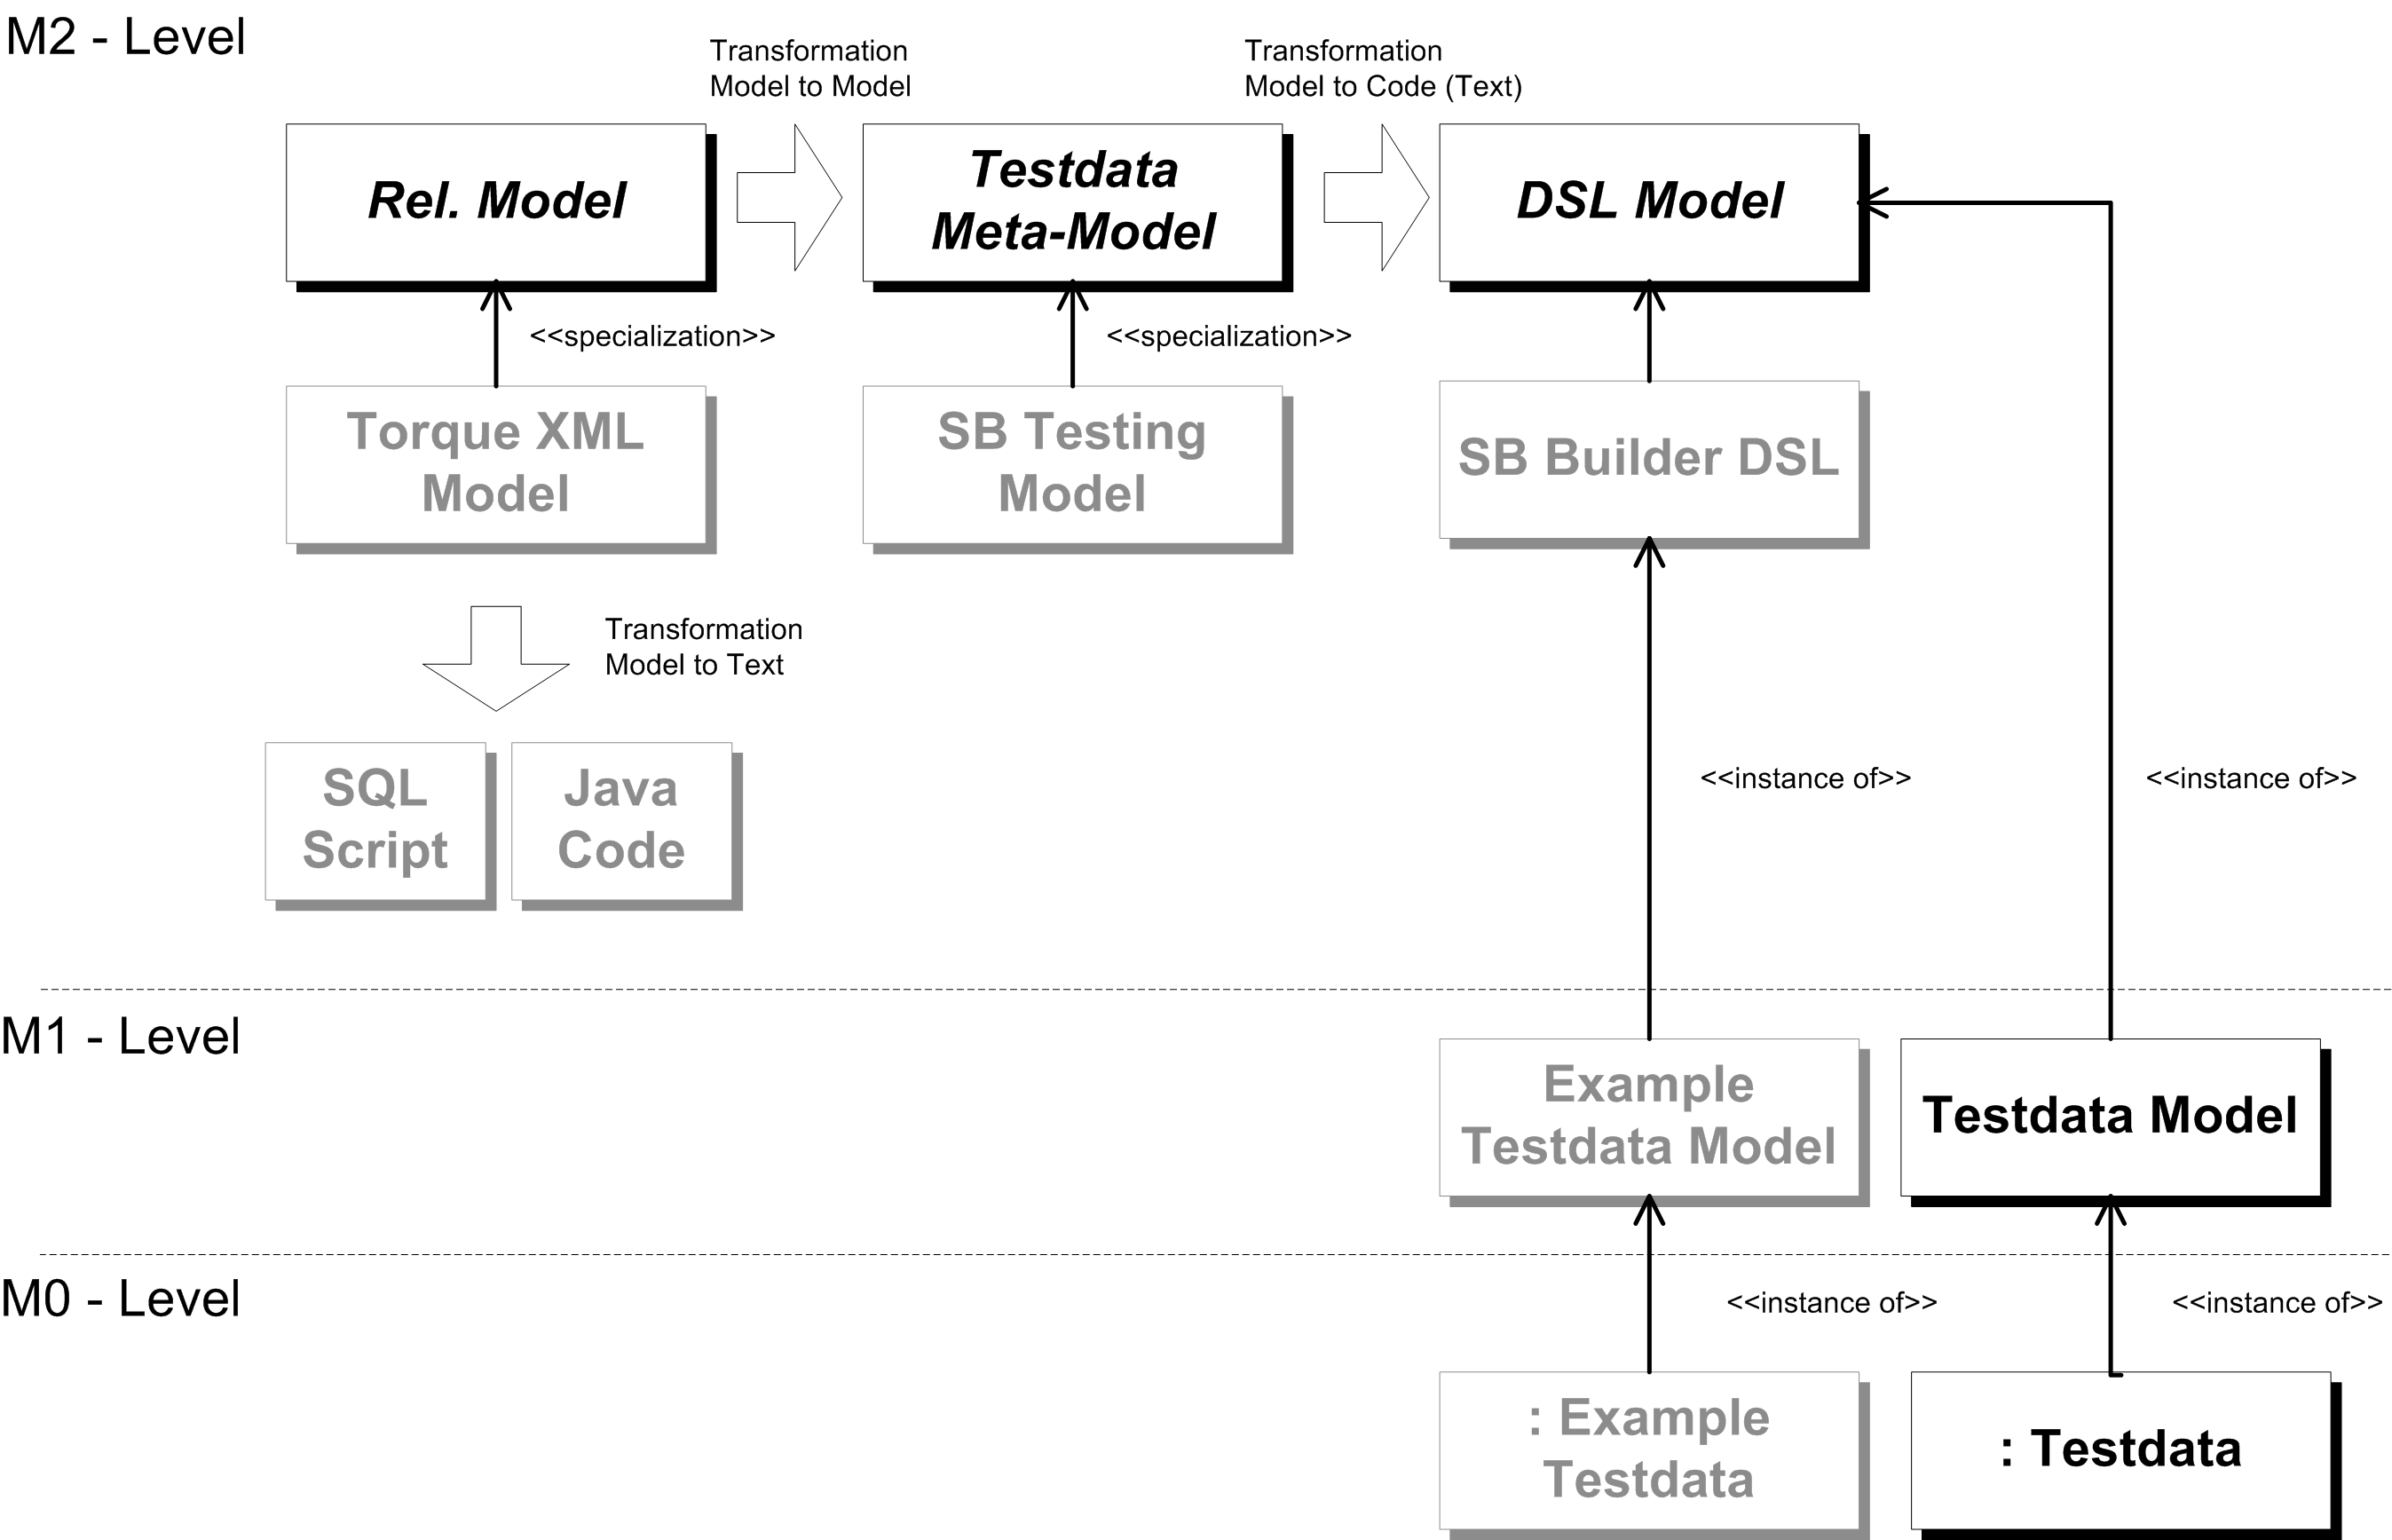
\includegraphics[width=0.95\textwidth]{images/grundlagen/sb_testing_model.png}
	\caption{Modell-Beschreibung}\label{img:sbtestingmodel}
\end{figure}

Das SB-Testing-DB-Modell enth�lt keine Datenbank-Constraints. Eine Abbildung dieser w�rde keine wesentliche Vorteile bringen. Das API
bzw. die erzeugten DataSets sind ausschlie�lich f�r den Einsatz im Test-Umfeld gedacht. Sollte ein DataSet Daten enthalten, die gegen 
die in der Datenbank definierten Constraints versto�en, scheitert das Einspielen des DataSets in die Datenbank und eine Fehlermeldung
wird ausgel�st.
Aus Sicht des Testers ist dieses Verhalten ausreichend, da die Exception zum Scheitern der Unit-Tests f�hren wird. Der Mehrwert,
dass ung�ltige DataSets schon vor dem Einspielen als solches zu erkennen, ist gering im Vergleich zu dem Aufwand, 
Constraint-Mechanismen verschiedener Datenbanksysteme nachzubauen.

Der Generator nutzt f�r die Code-Generierung \textit{Apache Velocity}. Velocity ist eine Template-Engine, die Dokumente mit Hilfe von
Templates erzeugt. Diese Templates bestehen aus Text und besonderen Velocity-Anweisungen. Zu den Anweisungen geh�ren unter anderem
Platzhalter, die w�hrend der Generierung durch konkrete Werte ausgetauscht werden. Velocity bietet mit Verzweigungen und Schleifen
auch Anweisungen zur Steuerung der Generierung.

Templates Dokumente erzeugt. Die Vorlagen k�nnen Platzhalter enthalten, die von Velocity durch konkrete Werte ausgetauscht werden, und
auch von Velocity interpretierte Steueranweisungen, z.B. Verzweigungen und Schleifen.



Die Namen der generierten Klassen h�ngen vom Modell ab. Unter anderem werden Klassen der folgenden Kategorien erzeugt:
\begin{itemize}

	\item \textbf{DataSet}: Es wird eine abstrakte DataSet-Klasse generiert. Der Zugriff auf die Tabellen erfolgt �ber �ffentliche
	  Felder. Die Klasse enth�lt die Methode \texttt{createDBUnitDataSet}, um die f�r die Unit-Tests ben�tigten DbUnit-DataSets zu
		erzeugen. Dabei werden Template-Methoden definiert, die genutzt werden k�nnen, um in den Erzeugungsprozess von DataSets
		einzugreifen. Die Klasse enth�lt dar�ber hinaus Methoden zum Hinzuf�gen von Zeilen in die entsprechende
		Tabellen.

	\item \textbf{Table}: F�r jede Tabelle wird eine entsprechende Klasse generiert. Der Klassenname setzt sich aus dem Namen
	  der Tabelle und dem Suffix "`Table"' zusammen. Die Klasse stellt Methoden zum Modellieren der Daten und f�r den Zugriff
		auf Tabellenzeilen bereit. 
		Einzelne Tabellenzeilen werden von einer passenden RowBuilder-Klasse repr�sentiert.
		Damit die Klasse direkt zur Erstellung von DbUnit-DataSets verwendet werden kann, implementiert sie das DbUnit-Interface
		\texttt{ITable}.
	
	\item \textbf{RowBuilder}: Zu jeder Tabelle wird eine Klasse zur Repr�sentation einer Tabellenzeile generiert. Die Klasse
	  beinhaltet f�r jede Spalte mehrere Methoden zum Setzen und Abfragen des jeweiligen Wertes. Die Methodennamen setzen sich
		zusammen aus der Aufgabe (\texttt{get} bzw. \texttt{set}) und dem Spaltennamen. \todo{Raw-Setter erkl�ren?}
	
	\item \textbf{FindWhere}: F�r einfache Suchanfragen gibt es f�r jede Tabelle die innere Klasse \texttt{FindWhere}. Sie erm�glicht
	  die Suche nach  einem Wert in einer Spalte und liefert eine Liste von Tabellenzeilen. Die Methode ist zur Suche nach Zeilen
		vorgesehen, von denen erwartet wird, dass es sie gibt. Passt keine Zeile zum Suchkriterium gefunden, wird eine
		Exception ausgel�st.
	
\end{itemize}

\todo{Bild mit Text integrieren}

\begin{figure}[H]
  \centering
	 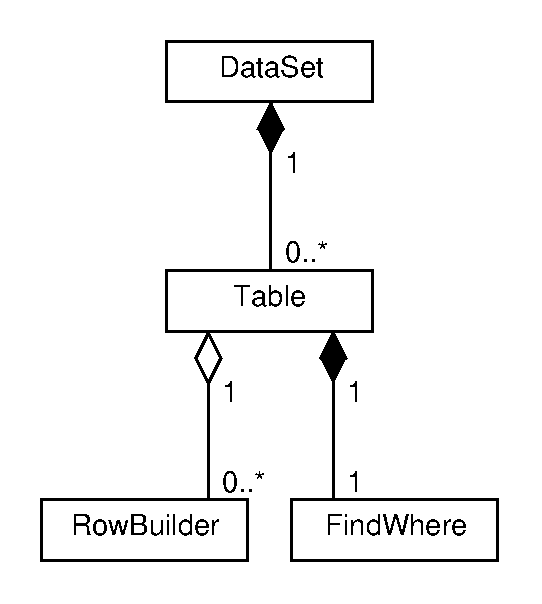
\includegraphics[width=0.4\textwidth]{images/grundlagen/sb_testing_classes.pdf}
	\caption{UML-Klassendiagramm der SB Testing DataSet Klassen}\label{img:sb_testing_classes}
\end{figure}




\section{Konventionen}
\label{sec:grundlagen:konventionen}

	\subsection{Datenbank ER-Diagramme}
	\label{sec:grundlagen:konventionen:datenbankdiagramme}
	F�r die Darstellung von Datenbank-Diagrammen wird ein einheitlicher Stil verwendet. Dieser orientiert sich an
	Ambler aus \cite{REFACTORING_DATABASES}. Auf die Angabe von Stereotypen wird sowohl bei den Tabellen, als auch
	bei den Beziehungen zwischen Tabellen verzichtet.
	
	Erkl�ren:
	- Spalten/PK/FK
	- Kardinalit�ten
	
	- basiert auf UML, Stereotypen bei Tabelle und Beziehungen weggelassen, 
	
	Abbildung \ref{img:ambler_table} zeigt ein Diagramm mit zwei Tabellen. Tabelle 2 enth�lt einen Fremdschl�ssel,
	der einem Prim�rschl�ssel aus Tabelle 1 

	\begin{figure}[H]
		\centering
		 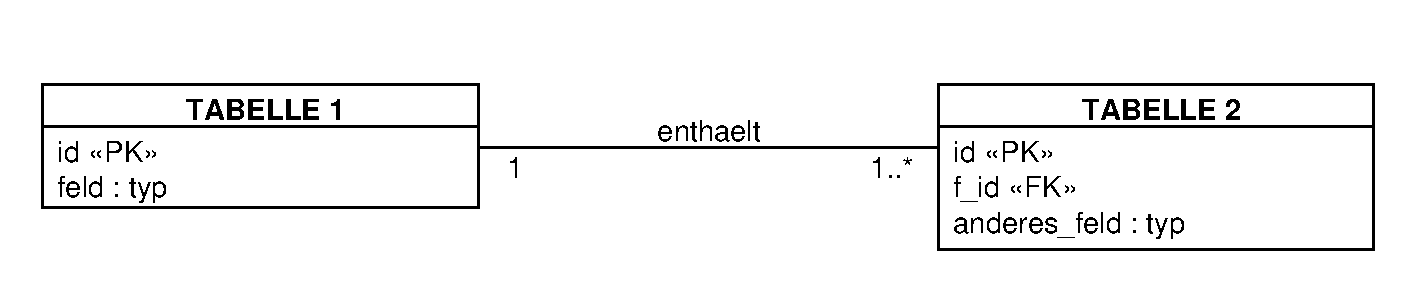
\includegraphics[width=0.75\textwidth]{images/grundlagen/ambler_table.pdf}
		\caption{Datenbank-Diagramm-Stil nach Ambler}\label{img:ambler_table}
	\end{figure}


	\chapter{Generierung von Testdaten}
\label{chap:generierungvontestdaten}

  \chapter{Zusammenfassung und Ausblick}

\todo{Zusammenfassung und Fazit schreiben}

- Kurze Zusammenfassung: Was wurde erreicht

- Offene Punkte / Weiterführende Arbeiten
  \chapter*{Titel}
\label{chap:titel}

\section*{Untertitel}
\label{Titel:�btertitel}


\subsection*{Stichpunkte}
\begin{itemize}
	\item
		\textbf{Item 1}: 
		Text

	\item
		\textbf{Item 2}: 
		Text
	
\end{itemize}


\subsection*{Aufz�hlung}
\begin{enumerate}
	\item
		\textbf{Item 1}: 
		Text

	\item
		\textbf{Item 2}: 
		Text
	
\end{enumerate}

\subsection*{Abk�rzung}
\nomenclature{GUI}{Graphical User Interface (Grafische Benutzeroberfl�che)}


\subsection*{Quellcode}
\begin{lstlisting}[caption=Der Titel, label=listing:label]
Code
\end{lstlisting}

\subsection*{Verweise}
\begin{enumerate}
	\item siehe \ref{listing:label}
	\item \reflst{listing:label}
	\item \refabb{img:imagelabel}
	\item \refsec{Titel:�btertitel}
	\item \refchap{chap:titel}
\end{enumerate}

\subsection*{Zitate}
\begin{enumerate}
	%\item \cite{MANUAL_ID}
	\item \cite{DSLS_IN_ACTION}
	\item \cite{REFACTORING_DATABASES}
	\item \cite{BASISWISSEN_SOFTWAETEST}
	\item \cite[20ff]{DER_INTEGRATIONSTEST}
	\item \cite{XUNIT_TEST_PATTERNS}
	\item \cite{DOMAIN_SPECIFIC_LANGUAGES}
	\item \cite{MODELLGETRIEBENE_SOFTWAREENTWICKLUNG}
\end{enumerate}

\subsection*{Bild}
\begin{figure}[H]
	\centering
	 
\includegraphics[width=0.8\textwidth]{images/cover/htwg_logo.png}
	\caption{Der Titel}\label{img:imagelabel}
\end{figure}


\subsection*{Bildgruppe}
\begin{figure}[htbp]
	\centering
	\subcaptionbox{Text 1\label{img:imagelabelX:image1}}[0.32\textwidth]{
		 
\includegraphics[width=0.32\textwidth]{images/cover/htwg_logo.png}
	}
	\subcaptionbox{Text 2\label{img:imagelabelX:image2}}[0.32\textwidth]{
		 
\includegraphics[width=0.25\textwidth]{images/cover/htwg_logo.png}
	}
	\subcaptionbox{Text 3\label{img:imagelabelX:image3}}[0.32\textwidth]{
		 
\includegraphics[width=0.16\textwidth]{images/cover/htwg_logo.png}
	}
	\caption{Gemeinsamer Titel}\label{img:imagelabelX}
\end{figure}




  
  \phantomsection % n�tig damit das Tabellenverzeichnis korrekt verlinkt wird
  \cleardoublepage
  \printnomenclature
  %\addcontentsline{toc}{chapter}{Abk�rzungsverzeichnis}
  

  %% Abbildungsverzeichnis generieren
  \phantomsection  % n�tig damit das Abbildungsverzeichnis korrekt verlinkt wird
  \cleardoublepage
  \listoffigures
  %\addcontentsline{toc}{chapter}{Abbildungsverzeichnis}
  
  %% Listingverzeichnis generieren
  \phantomsection  % n�tig damit das Listingverzeichnis korrekt verlinkt wird
  \cleardoublepage
  \lstlistoflistings
  %\addcontentsline{toc}{chapter}{Listings}
  
  %% Tabellenverzeichnis generieren
  %\phantomsection % n�tig damit das Tabellenverzeichnis korrekt verlinkt wird
  %\cleardoublepage
  %\listoftables
  %\addcontentsline{toc}{chapter}{Tabellenverzeichnis}

  %% Literaturverzeichnis generieren
  \phantomsection  % n�tig damit das Literaturverzeichnis korrekt verlinkt wird
  \cleardoublepage
  \printbibliography  
  %m\addcontentsline{toc}{chapter}{Literaturverzeichnis}

  %% Abschnitt fuer den Anhang
  \begin{appendix}
  \end{appendix}
	
	\todos
\end{document}